\documentclass{article}
\usepackage[utf8]{inputenc}
\usepackage{graphicx}
\usepackage{lipsum}
\usepackage{float}
\usepackage{pdfpages}
\usepackage{lineno, blindtext}

\usepackage[margin=1in,left=1.5in,includefoot]{geometry}

% code snippets setup
\usepackage{listings}
\usepackage{color}

\definecolor{dkgreen}{rgb}{0,0.6,0}
\definecolor{gray}{rgb}{0.5,0.5,0.5}
\definecolor{mauve}{rgb}{0.58,0,0.82}

\lstset{frame=tb,
  language=C,
  aboveskip=3mm,
  belowskip=3mm,
  showstringspaces=false,
  columns=flexible,
  basicstyle={\small\ttfamily},
  numbers=left,
  numberstyle=\tiny\color{gray},
  keywordstyle=\color{blue},
  commentstyle=\color{dkgreen},
  stringstyle=\color{mauve},
  breaklines=true,
  breakatwhitespace=true,
  tabsize=3
}
%

% Header and Footer
\usepackage{fancyhdr}
\pagestyle{fancy}
\fancyhead{}
\fancyfoot{}
\fancyfoot[R]{ \thepage\ }
\renewcommand{\footrulewidth}{0pt}
%


\begin{document}

% title page content
\begin{titlepage}
    \begin{center}
        
\includegraphics[height= 4cm ]{UoRlogo.png} \\
        [5mm]
        \textsc{\Large University of Reading} \\
        [0.5cm]
        \textsc{\Large Department of Computer Science} \\
        [1cm]

        \line(1,0){300}\\
        [0.25in]
        \huge{\bfseries Extending a Platform Game in C/CC++: User Experience Enhancement}\\
        [2mm]
        \line(1,0){200} \\
        [1cm]
        \textsc{\Large Jason Jay Dookarun} \\
        [2mm]
        \textsc{\large Word Count: 2225 } \\
        [0.2mm]
        \textsc{\large (Excluding Diagrams and Code Snippets)}\\
        [2mm]
        \textsc{\large Page Count: 25}\\
        [4cm]
        \end{center}
        \begin{flushright}
        \textsc{\normalsize Module Code: CS1PR16 \\
        Assignment Report Title: Programming Project \\
        Student Number: 26017434 \\
        Time Spent: 50 Hours \\
        April 21, 2020 } \\
        \end{flushright}
\end{titlepage}

% front matter
\pagenumbering{roman}
\section*{Summary}
\addcontentsline{toc}{section}{\numberline{}Summary}

The following document consists of an in-depth systematic examination of elements developed by I, Jason Jay Dookarun, to an existing C/C++ program developed by Parallel Realities. The given program is a platform game that employs the SDL2 library for the demonstration of graphics. A feature has been composed, modified and extended, integrated within the provided game, with the support provided by the skeleton code, authorised by \textbf{Dr Julian Krunkel} of the Department of Computer Science at the University of Reading. The aforementioned will further elaborate on the procedures undertaken to develop the feature(s) including design illustrations, methods of implementation and development process.

\section*{Declaration}
\addcontentsline{toc}{section}{\numberline{}Declaration}

I, \textbf{Jason Jay Dookarun}, of the Department of Computer Science at the University of Reading, confirms that all the sentences, figures, tables, equations, code snippets, artwork and illustrations in this report are original and have not been taken from any other person’s work, except where the works of others have been explicitly acknowledged, quoted and referenced. I understand that if failing to do so will be considered as a case of plagiarism. Plagiarism is a form of academic misconduct and will be penalised accordingly.

    \begin{flushright}
    \textbf{Jason Jay Dookarun} \\
    April 21, 2020\\
    [1cm]
    \end{flushright}

\cleardoublepage
\tableofcontents
\thispagestyle{empty}
%\cleardoublepage

\listoffigures
\addcontentsline{toc}{section}{\numberline{}List of Figures}
\cleardoublepage





\newpage
\section{Introduction}\label{sec:intro}
\rhead{Introduction}
\lhead{Extending a Program in C/C++}
The provided program employs an SDL2 library to illustrate graphical components, coded in C/C++. This program has been developed and created by Parallel Realities titled "Pete's Pizza Party 6". The present project has been produced using the SDL2 library setup. The current game enables a user to control a sprite to collect all objects illustrated on the screen appropriately before the termination of the game.

\subsection{Project Goals}
This project aims to develop an extension to the existing piece and further describe the choice made and implementation cycle applied. Authorised by the academic staff members at the University of Reading, I was provided with a skeleton code containing sections of the existing platform game, namely "Pete's Pizza Party 6".

\subsection{Game Features}
The aim of the game entails accumulating all objects positioned across disparate seconds of the map. These objects would be portrayed as pizza slices. As the user assembled every pizza slice, the HUD, located on the right-hand side of the user's screen, would increment, accordingly. Once the entity collected all the elements, the game would be terminated.
\begin{figure}[H]
    \centering
    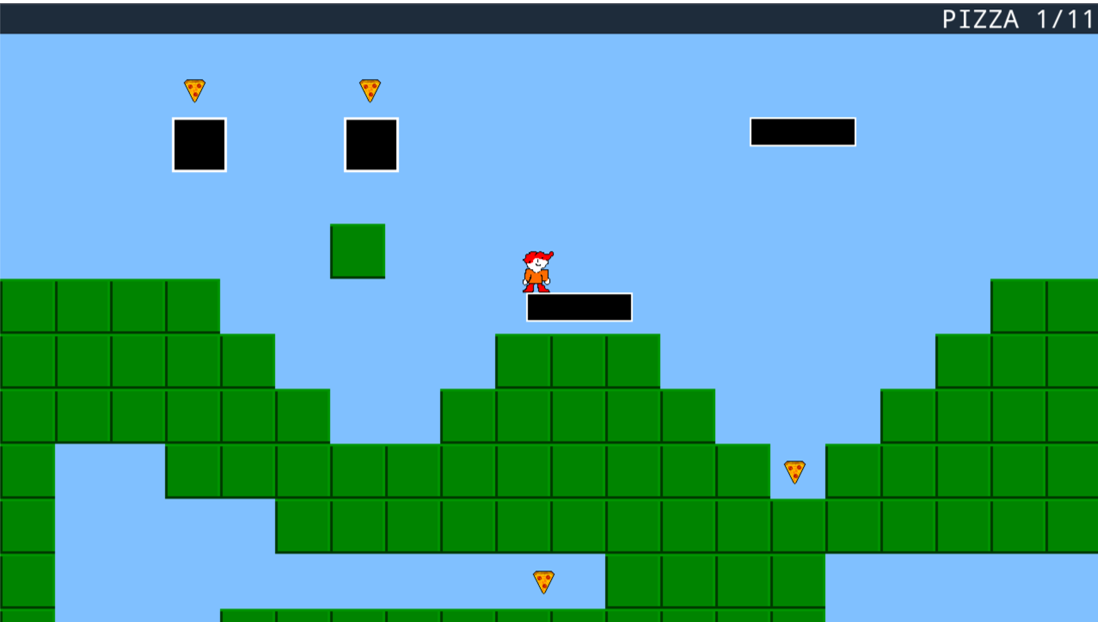
\includegraphics[height=3in]{figure1.png}
    \caption[Pete's Pizza Party: Pre-Extension]{Pete's Pizza Party: Pre-Extension}
    \label{fig:pete's pizza party}
\end{figure}
After running several instances, I was able to identify numerous components that could've been adjusted or implemented to provide the user with enhanced user experience, namely universal control commands, a support panel and an introduction sequence to allow the user to comprehend the product.

Currently, the product implements any player movement the use of the letters A, D, I and SPACE, where A represents a movement to the left, D represents a movement to the right, I represents jump, and SPACE represents a reset functionality. This could be potentially identified as a difficulty for the user, as a universal control panel is not implemented. Moreover, no support is provided to the user for one to understand what the controls may be. This sector can, as a result, be identified as a weakness, allowing such an extension to be provided.

Moreover, once the program is executed, the user is immediately provided with the main program. As a result, the user is not provided with a formal welcome to the game and intricately links to the avoidance of positive user experience. Furthermore, once the user does complete collecting all objects displayed on the map, the user is not provided with an option to play again, but instead is forced to view the game terminated. Both of the raised weaknesses interlink with the subject of user experience, as both consequently do not fulfil positive UX (User Experience) for the user. This, as a consequence, provided me with a segment to converge upon, to transform and intensify the product for future clientele.

\subsection{Programming Style}
To achieve my modifications, I originated by performing a bottom-up approach. \cite{bottom-up} A bottom-up method fulfils modifications commencing with the evaluation of existing components within the program, followed by constructing more complex features. This can be considered as an asset as it reuses existing methods, eradicating the need for additional examination. I will be programming in C throughout the course of the project to inject my modifications coherently.


\section{Design}\label{sec:design}
To coherently comprehend the flow of a project, it is important to implement a design structure, whereby one can visualise before building or modifying any designated section. Moreover, to ensure that the project is understandable, levels of abstraction can be implemented at levels like design, allowing communication to take place between teams.



\subsection{Feature Design}
Following my brief analysis of the program before development, I believe that it would be useful to focus on changes correlating to one's perception of the user's experience. This would include an introductory screen to welcome the user, implementing an in-game support mechanism, to further support the user during live game-play.  Moreover, modifications are to be made to the controls the player must follow, to adhere to a universal control method. Finally, a closing progression would be performed to allow the user to either: play the game again or exit the game appropriately, as an alternative to a forceful closure by the machine.

\subsection{Gameplay after Modification}
Once these modifications have been added, the game would commence from the main introductory screen as an alternative to the main gameplay screen. This would act as a welcome panel for the user, to comprehend the game as well as controls before playing. Once the user presses SPACE, the game will initiate as usual.

New controls are to be executed to follow a WASD or Up Down Left Right universal control setup. Once the game is finished, the user will then be shown an outro screen, presenting them with a possibility to either restart the game or exit the game, as an alternative to a force stop. New features are to be implemented, whereby the user can exit the game at any stage as well as an option to view controls via a key command.

\subsection{Illustrative Design}
To symbolise my concepts appropriately, I selected to further complete research in such fields. This would allow me to comprehend where to insert my modifications to positively impact both the project, as well as the client. Diverse techniques can be used to learn where changes should be added, including methods like UML diagrams and flowcharts.
\rhead{Design}
\subsubsection{Flowchart}\label{sec:flowcharts}
A flowchart is defined as "a diagram that depicts a process, system or computer algorithm." A flowchart can be utilised in a countless number of ways, as mentioned above. Similar to methods depicted both in UML diagrams and pseudocode, a flowchart illustrates a physical construct on how one may define their "algorithm".  To comprehend how a flowchart functions, a universal keyset it used, for future users to understand its meaning. For instance, in the format of flowcharts, diamonds often refer to a decision that one must take. Such structures can be of effective use, as it allows one to experience the flow of a project in a digital and directed manner.

\begin{figure}[H]
    \centering
    \includegraphics[height=3.5in]{introflowchart.png}
    \caption[Introduction Flow Chart]{Introduction Flow Chart}
    \label{fig:flowchart}
\end{figure}

As illustrated above, the flowchart implements my modifications that are to be executed. This solely focuses on the true nature of the introductory page that will be created. As pointed, numerous sections are given to the user through commands. These examples include pre-set reactions by the machine to key presses. This permits the formation of fluidity to the system, including a process of adhering to the user's experience.


\subsubsection{UML Diagram}\label{sec:uml}
UML diagrams can be utilised as a form of representation, allowing a way of "visualizing a software program using a collection of diagrams." \cite{UML} A UML diagram can be useful by illustrating how objects interlink with one another.  Likewise, in such scenarios, this enables me to learn the accurate position to infuse my advancements and modifications.

\begin{figure}[H]
    \centering
    \includegraphics[height=3.5in]{uml.png}
    \caption[UML after Modifications]{UML after Modifications}
    \label{fig:uml}
\end{figure}

As illustrated in Figure 3, the new modifications would effectively implement a new introduction sequence and an outro sequence. Effectively, all the sectors in the main section are inherited from alternative sections as illustrated. On the other hand, the outro sequence and intro sequence will inherit similar features as one another.

\section{Implementation and Development}
As discussed in the design section, my modifications are to be specifically tailored to the user's experience. This includes the addition of an introductory panel for the user to be welcomed by, a modification in the controls sector by adding a universal control set, and an outro sector, providing the user with an opportunity to exit the game appropriately or replay.

To effectively implement my modifications, I began by applying the bottom-up approach as my principal methodology. This enabled me to modify existing sections, ensuring that both the program would resume working and certain sectors could be efficiently reused, thus reducing further testing. As a result, my initial segment of progress converged upon the control panel as this was a current section implementing minor modifications.

An immediate modification that was made to the game was the renaming on the program from "Pete's Pizza Party 6" to "Pete's Pizza Hunt". This provided a unique name to match the game accordingly. Graphics for both introductory panels and outros were designed through the use of Adobe PhotoShop CC.
\begin{figure}[H]
    \centering
    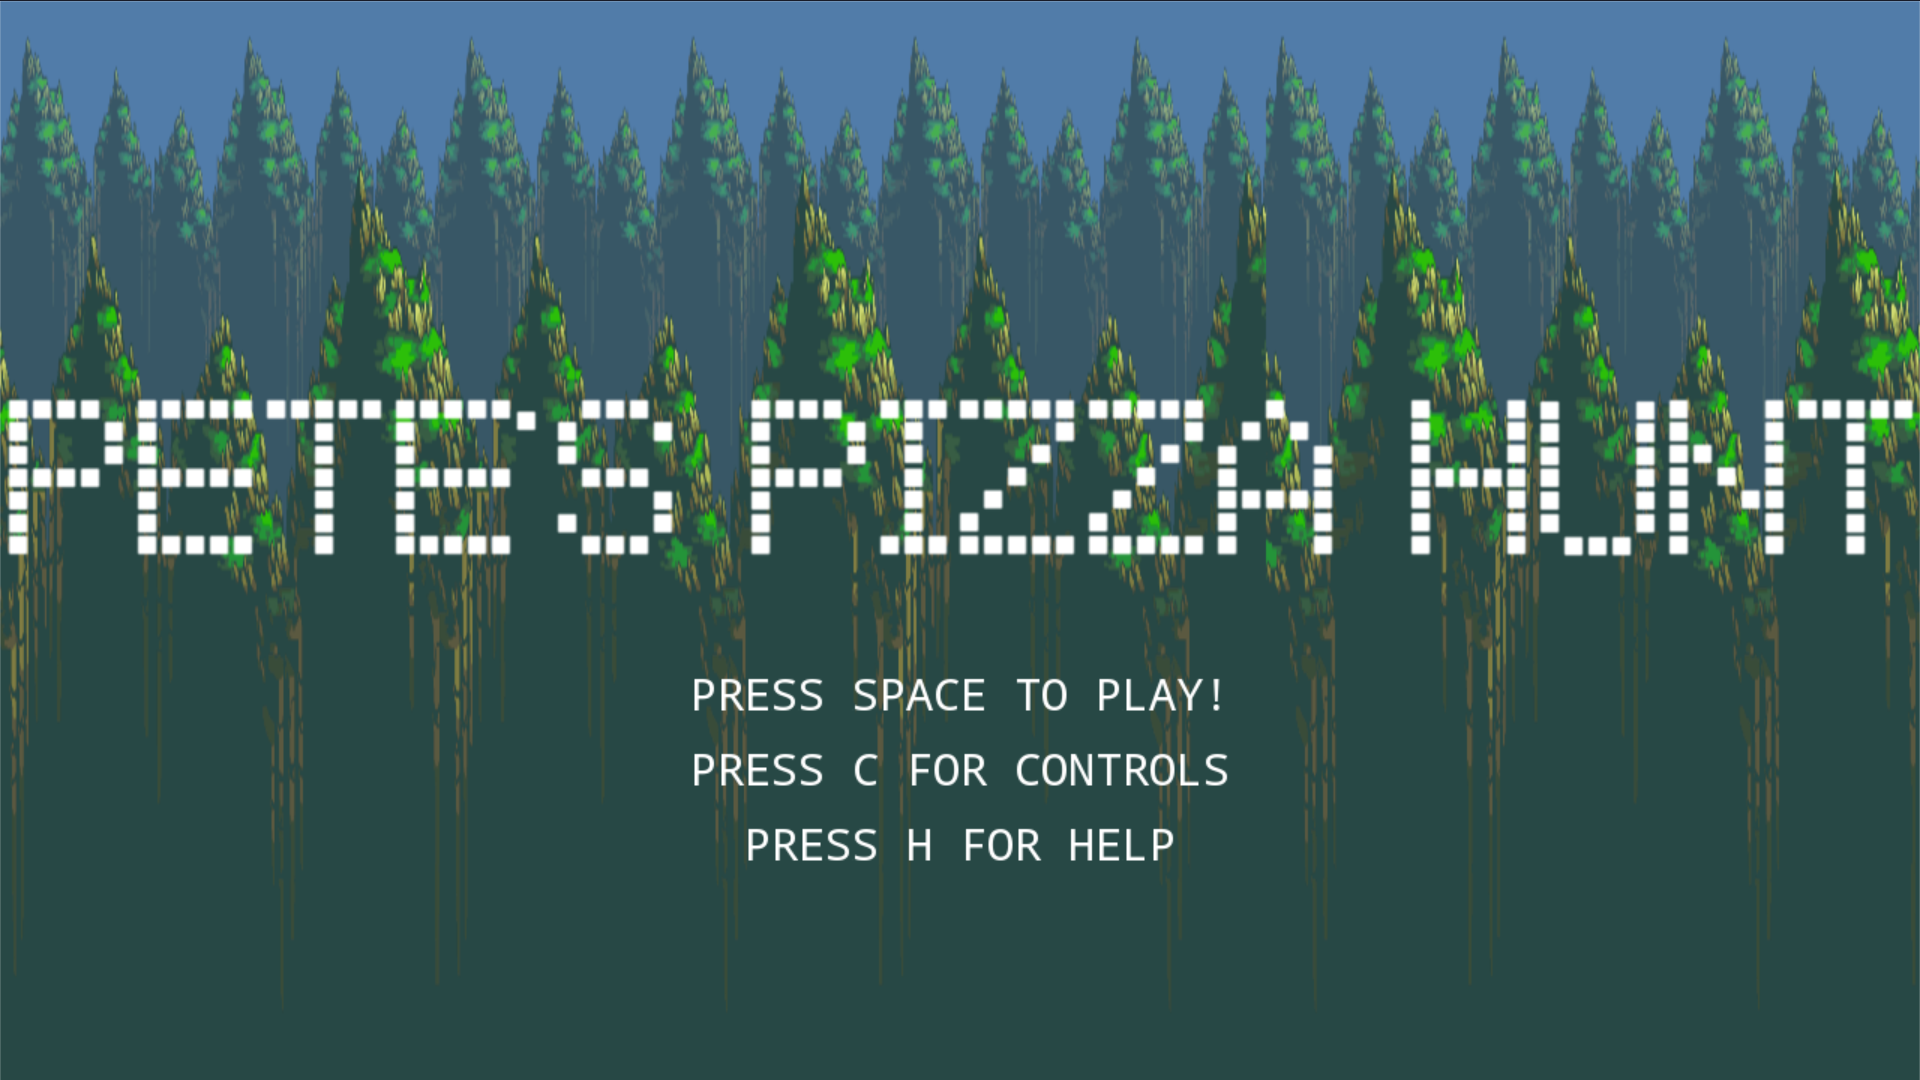
\includegraphics[height=3in]{intro.png}
    \caption[Introduction Screen]{Introduction Screen}
    \label{fig:flowchart}
\end{figure}

\subsection{Control Panel Modifications}
To efficiently implement the new universal control methods, it was crucial to distinguish the present methods that were being employed in the program. Firstly, I started by examining the existing player.c file confined in the game, pre-development. This contained commands that the client was to be applying throughout the course of the game, before modifications to move the sprite.
\begin{lstlisting}[caption={player.c Initial Code},captionpos=b]
void doPlayer(void)
	if (app.keyboard[SDL_SCANCODE_A]){
		player->dx = -PLAYER_MOVE_SPEED;
		player->texture = pete[1];
\end{lstlisting}
As illustrated by listing 1, the existing methods contained within the program illustrated the use of the key A and the key D, as shown by lines 5 and 8. Once these keys were to be pressed, the system would react in a designated method, i.e. move left or move right. This, as a result, provided me with an appropriate platform to implement changes.
\begin{lstlisting}[caption={player.c Modifications},captionpos=b]
if (app.keyboard[SDL_SCANCODE_LEFT])
	{
		player->dx = -PLAYER_MOVE_SPEED;
		player->texture = pete[1];
	}
\end{lstlisting}
Following the existing methods, I was able to apply the appropriate modifications by changing the scan-code to the appropriate key. This permitted the user to be provided with 2 manners of controlling the sprite, via WASD control method or the use of the Up Down Left and Right key prompts, accordingly (see Appendix B). This method was of extreme use as it allowed me to develop further configurations to benefit the player, later discussed. To ensure that testing was performed accordingly, the game was executed over numerous cycles to ensure performance was maintained accordingly. \rhead{Implementations and Development}
\subsection{Introductory "Splash" Screen Creation}
Once the modified controls were completed, I commenced working upon the introduction sequence. To understand how one may create this, I referenced the work and tutorial developed by Parallel Realities. This would allow me to understand what stages were required. This section, similar to stage.c required 3 concepts, logic(void), draw(void) and init() sequence. Similar to initstage(), initTitle() could be formulated identically to annul complications. With regards to the draw, the sector would implement the creation of the main screen as a platform to further build upon. As illustrated, lines 3-6 generate the panel for display, followed by line 7 formulating a render.
\begin{lstlisting}[caption={homescreen.c background setup},captionpos=b]
// implements the drawing of the wallpaper onto the screen
	for (x = existingBackground; x < SCREEN_WIDTH; x += SCREEN_WIDTH){
		screen.x = x;
		screen.y = 0;
		screen.w = SCREEN_WIDTH;
		screen.h = SCREEN_HEIGHT;
		SDL_RenderCopy(app.renderer, background, NULL, &screen);
	}
\end{lstlisting}
Once this section successfully executed, further modifications were applied such as a control mechanism to take the user from one screen to another. The initial process involved designing/writing a message on the existing platform as shown below:
\begin{lstlisting}[caption={homescreen.c command prompts},captionpos=b]
loadText(logo, &r, (SCREEN_WIDTH / 2) - (r.w / 2), 250);
	// projected onto wallpaper as a visible instruction
	drawText(SCREEN_WIDTH / 2, 450, 255, 255, 255, TEXT_CENTER, "PRESS SPACE TO PLAY!");
	drawText(SCREEN_WIDTH / 2, 500, 255, 255, 255, TEXT_CENTER, "PRESS C FOR CONTROLS");
	drawText(SCREEN_WIDTH / 2, 550, 255, 255, 255, TEXT_CENTER, "PRESS H FOR HELP");
\end{lstlisting}
As demonstrated by the codes, the system requires the user to select a set of control to respond. Similar to the design section, such could be achieved by providing the user with a message box, and thus was implemented.
\begin{lstlisting}[caption={homescreen.c messsage boxes},captionpos=b]
void messageboxC(void) {
	// referenced from https://wiki.libsdl.org/SDL_ShowMessageBox#Version
		const SDL_MessageBoxButtonData buttons[] = {
	{ SDL_MESSAGEBOX_BUTTON_RETURNKEY_DEFAULT, 0, "OK" },
	};
		const SDL_MessageBoxData messageboxdata = {
		SDL_MESSAGEBOX_INFORMATION,NULL,"Controls","Left: LEFT Key or A, Right : RIGHT Key, Jump : SPACE or W, Reset : R, Quit : Q.",SDL_arraysize(buttons),buttons };
	int buttonid;
	if (SDL_ShowMessageBox(&messageboxdata, &buttonid) < 0) {
		SDL_Log("error displaying message box");
		return 1;
	}
	if (buttonid == 0) {
		return;
	}
}
\end{lstlisting}
\rhead{Implementation and Development}

\subsection{Outro Screen Creation}
Similarly, by using methods applied within the introductory section, I developed an identical function to take place as an outro. This would specifically function in a manner whereby an alternative display will be shown to the user, with a new background soundtrack. This would be followed by a new command prompt allowing the user to 1) restart the game or 2) exit appropriately. Lines 4-5 initiate the processing of logic() and draw() prior to 7-8 loading content. Lines 11-12 initate the soundtrack and play the appropriate audio.
\begin{lstlisting}[caption={homescreen.c initTitle() sequence},captionpos=b]
// initiates the loading of the graphics and plays the background audio,
void initTitle(void)
{
	app.delegate.logic = logic;
	app.delegate.draw = draw;
	// this allows the background wallpaper to be uploaded and displayed for the user.
	background = loadTexture("gfx/backgroundNew.png");
	logo = loadTexture("gfx/logo.png");
	// the music score utilised in the introduction package is an adaptation of Stu Phillips' Knight Rider Theme, covered by
	// Jason Jay Dookarun and recorded.
	loadMusic("music/kr.mp3");
	playMusic(1);
}
\end{lstlisting}
\begin{lstlisting}[caption={outro.c initOutro() sequence},captionpos=b]
void initOutro(void)
{
	Mix_HaltChannel(-1);
	app.delegate.logic = logic;
	app.delegate.draw = draw;
	background = loadTexture("gfx/outro.png");
	logo = loadTexture("gfx/missionaccomplished.png");
	// Music from : https://www.bensound.com
	loadMusic("music/bensound-erf.mp3");
	playMusic(1);
}
\end{lstlisting}
As illustrated above, minor modifications were applied to both sections to ensure that both sections were to react in an appropriate manner, accordingly. Modifications further involved a change in procedures that followed following a key press as illustrated below:

\begin{lstlisting}[caption={outro.c Key Press Process},captionpos=b]
// restarts the game by transferring the client to the introductory splash screen
	if (app.keyboard[SDL_SCANCODE_P]) {
		initTitle();
	}
	// similar to homescreen.c, allows the user to meet the exit message box to confirm their decision.
	if (app.keyboard[SDL_SCANCODE_Q]) {
		messageboxYesNo();
	}
}
\end{lstlisting}
\rhead{Implementation and Development}

\subsection{In-Game Support Panel}
As previously explained, the control mechanisms were developed accordingly through the use of keypress prompts. To ensure the user understood the function of the game during live gameplay, existing keypress commands were injected. This would permit the user to regularly review any controls as well as exit the game if needed through an exit panel. This was processed and completed by injecting the controls message box into stage.c, (view listing 5). As illustrated below, the exit mechanism was developed via a message box setup. As demonstrated, lines 2-4 initiate a button setup, allowing the user to click accordingly. The data would then be recorded (via line 5) prior to providing a set reaction, as shown by lines 8-15.
\begin{lstlisting}[caption={Exit Message Box},captionpos=b]
void messageboxYesNo(void) {
	const SDL_MessageBoxButtonData buttons[] = {
	{ SDL_MESSAGEBOX_BUTTON_ESCAPEKEY_DEFAULT, 1, "Yes" },
	{ SDL_MESSAGEBOX_BUTTON_RETURNKEY_DEFAULT, 2, "No" },};
	const SDL_MessageBoxData messageboxdata = {
		SDL_MESSAGEBOX_INFORMATION,NULL,"Exit Game","Do you wish to exit the game?",SDL_arraysize(buttons),buttons };
	int buttonid;
	if (SDL_ShowMessageBox(&messageboxdata, &buttonid) < 0) {
		SDL_Log("error displaying message box");
		return 1;}
	if (buttonid == 1) {
		exit(0);}
	else {
		return;	}
}
\end{lstlisting}
As a result, the following would be presented to the user when a keypress command was to be activated during live gameplay.
\begin{figure}[H]
    \centering
    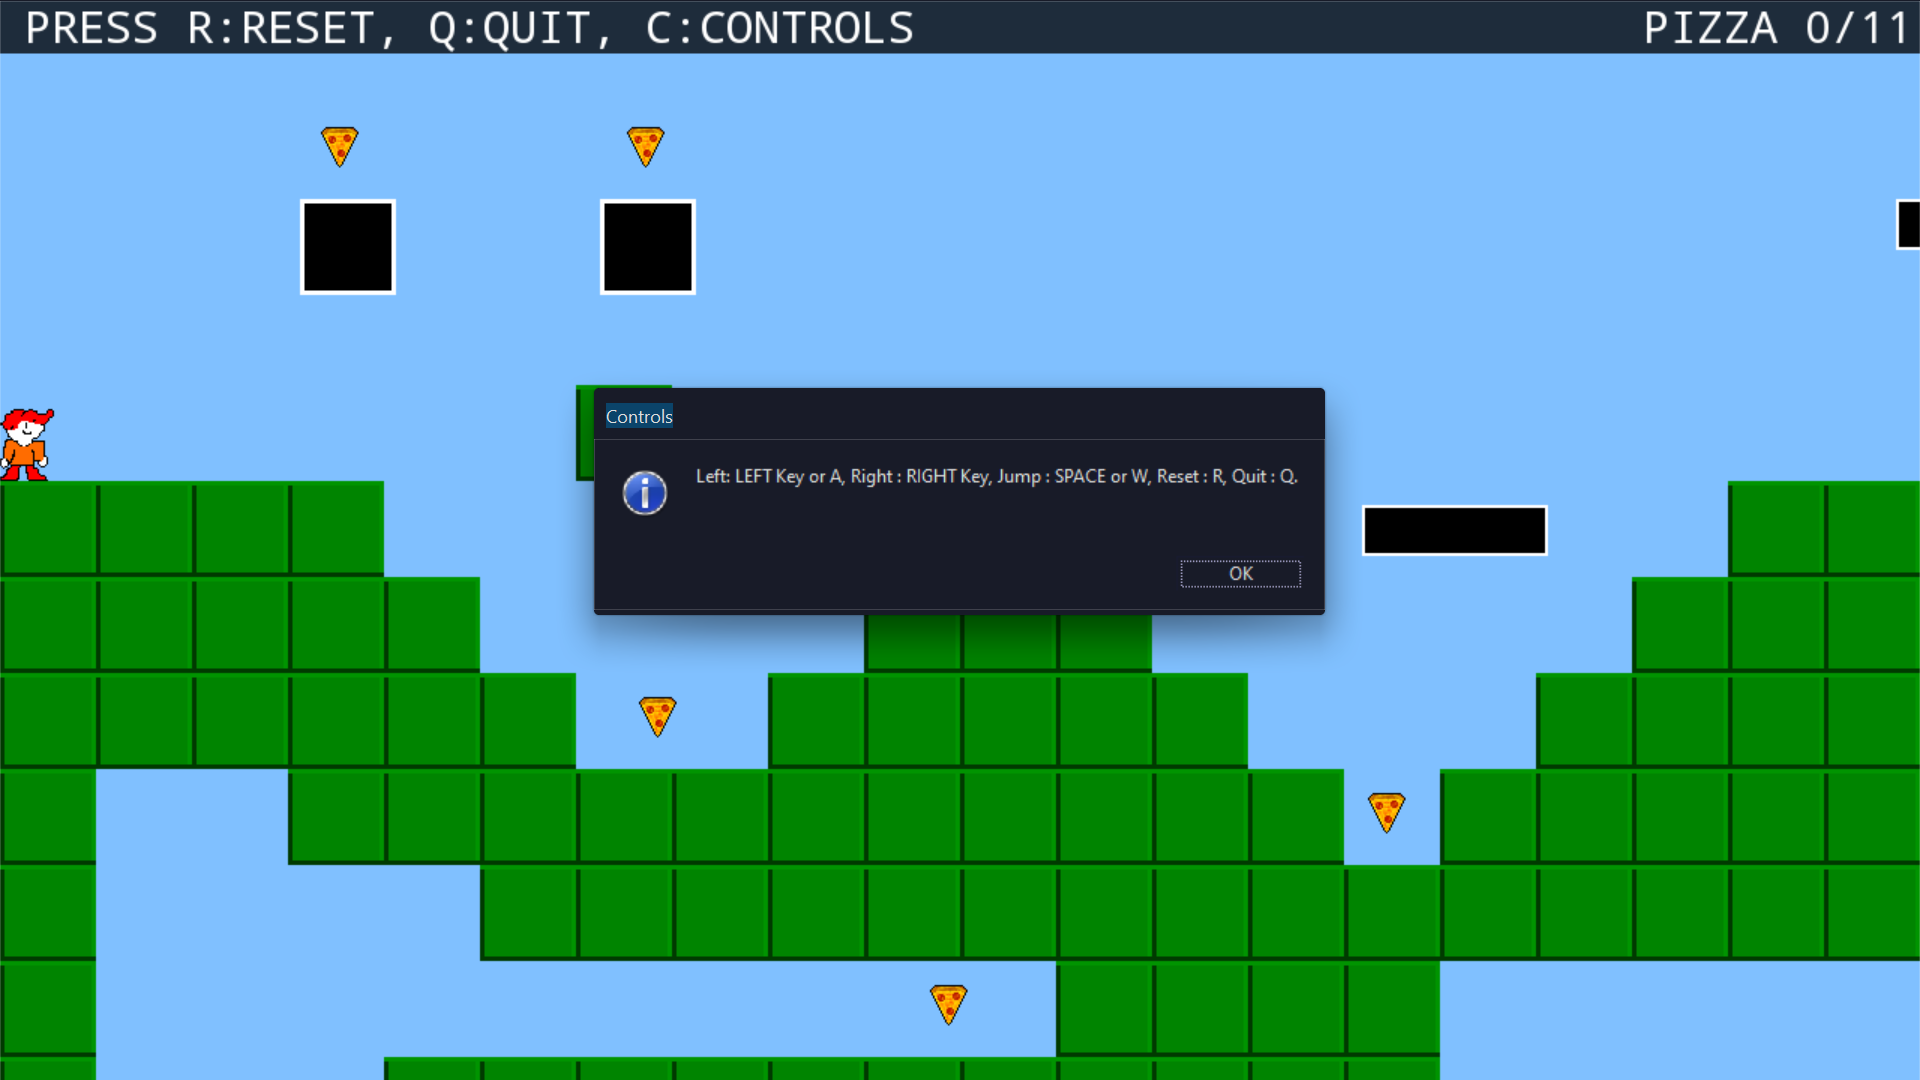
\includegraphics[height=2.1in]{ingamecontrol.png}
    \caption[In-Game Support]{In-Game Support}
    \label{fig:support}
\end{figure}

\section{Conclusion}
\rhead{Conclusion}
In conclusion, I believe that my modifications have improved one's perception of the product by applying new methods to improve engagement. By applying sound effects to the introduction sequence and text animations, it allowed for a vaster audience to be interested in the product.

Developing a significant program like the one provided allowed me to understand from a different viewpoint of a customer what features affect one's perception, as well as methods of implementation, through research and further learning. Likewise, this project allowed me to apply different fields of knowledge such as my studies of Software Engineering as well as Programming at the University of Reading. Moreover, given the time frame provided by academic members, I was able to effectively understand the importance of time throughout the course of this project. This project allowed me to utilise La-Tex as a production method to develop my report, and I believe that this would be a skill that I would implement regularly to ensure professionalism is maintained throughout my future documentations.

If provided further time, I would try to implement another level to the program and change the constraint from the number of pizzas to collect to a time constraint. This would effectively interlink into the creation of a high score leader-board to form a further competition between players.

If I was able to re-complete the project, I would aim to focus more time towards the start of the project instead of delaying modifications I added in. This would have resulted in me in having more time to develop further features.

\cleardoublepage

\begin{thebibliography}{9}
\rhead{References}

\bibitem{2DPlatform}
Parallel Realities,
\textit{2D Platformer Tutorial} \\
\texttt{https://www.parallelrealities.co.uk/tutorials/ppp/ppp1.php}

\bibitem{shootem}
Parallel Realities,
\textit{2D Shoot 'Em Up Tutorial} \\
\texttt{https://www.parallelrealities.co.uk/tutorials/shooter/shooter15.php}

\bibitem{bottom-up}
Bottom-Up Programming,
\textit{Bottom-Up Programming} \\
\texttt{https://bit.ly/2XE4JNs}

\bibitem{pseudo}
Science Direct,
\textit{Pseudocode} \\
\texttt{https://www.sciencedirect.com/topics/engineering/pseudocode}


\bibitem{MessageBox}
SDL Wiki 2.0,
\textit{SDL Message Box} \\
\texttt{https://wiki.libsdl.org/SDL_ShowMessageBox}

\bibitem{SimpleMessageBox}
SDL Wiki 2.0,
\textit{SDL Simple Message Box} \\
\texttt{https://wiki.libsdl.org/SDL_ShowSimpleMessageBox}


\bibitem{userexperience}
Don Norman and Jakob Nielsen,
\textit{The Definition of User Experience} \\
\texttt{https://www.nngroup.com/articles/definition-user-experience}

\bibitem{UML}
SmartDraw,
\textit{UML Diagram } \\
\texttt{https://www.smartdraw.com/uml-diagram/}

\bibitem{Flowchart}
Lucid Chart,
\textit{What is a Flowchart?} \\
\texttt{https://www.lucidchart.com/pages/what-is-a-flowchart-tutorial}

\bibitem{Abstraction}
Thorben Janssen, Stackify,
\textit{What is Abstraction?} \\
\texttt{https://stackify.com/oop-concept-abstraction/}


\end{thebibliography}
\cleardoublepage
\rhead{Appendix A}
\section{Appendix A: Full Flowchart}
\begin{figure}[H]
    \centering
    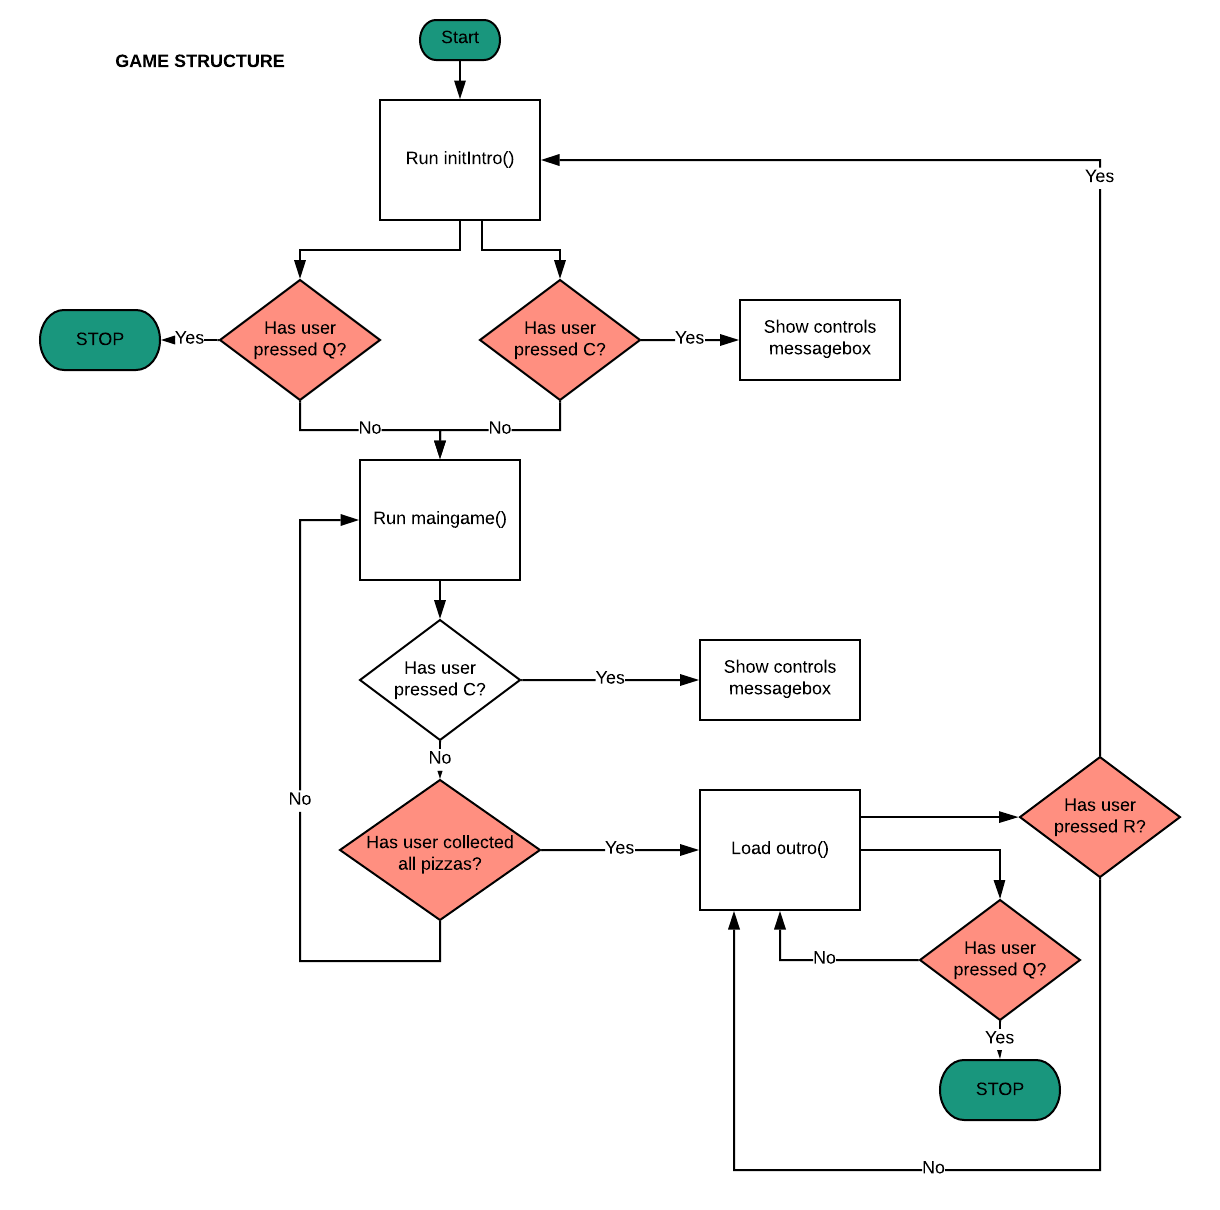
\includegraphics[height=7in]{flowchartfull.png}
    \caption[Flowchart]{Flowchart}
    \label{fig:Flowchart}
\end{figure}

\section{Appendix B: Code Changes}
Code Changes: https://csgitlab.reading.ac.uk/qt017434/CS1PR-Project

\includepdf[pages={1,2,3}]{gitlabrepo}


\section{Appendix C: Player.c After Modifications}
\begin{lstlisting}

void initPlayer(void)
{
	player = malloc(sizeof(Entity));
	memset(player, 0, sizeof(Entity));
	stage.entityTail->next = player;
	stage.entityTail = player;

	player->health = 1;

	pete[0] = loadTexture("gfx/pete01.png");
	pete[1] = loadTexture("gfx/pete02.png");
	player->texture = pete[0];
	SDL_QueryTexture(player->texture, NULL, NULL, &player->w, &player->h);
}

/* the section below implements the new commands for controlling the entity with appropriate control gestures such as WASD or UpDownLeftRight and SPACE
*/
void doPlayer(void)
{
	player->dx = 0;
	if (app.keyboard[SDL_SCANCODE_A])
	{
		player->dx = -PLAYER_MOVE_SPEED;
		player->texture = pete[1];
	}

	if (app.keyboard[SDL_SCANCODE_D])
	{
		player->dx = PLAYER_MOVE_SPEED;
		player->texture = pete[0];
	}
	if (app.keyboard[SDL_SCANCODE_W] && player->isOnGround)
	{
		player->riding = NULL;
		player->dy = -20;
		playSound(SND_JUMP, CH_PLAYER);
	}

	if (app.keyboard[SDL_SCANCODE_R])
	{
		player->x = player->y = 0;
		app.keyboard[SDL_SCANCODE_R] = 0;
	}

	// new code

	if (app.keyboard[SDL_SCANCODE_LEFT])
	{
		player->dx = -PLAYER_MOVE_SPEED;
		player->texture = pete[1];
	}

	if (app.keyboard[SDL_SCANCODE_RIGHT])
	{
		player->dx = PLAYER_MOVE_SPEED;
		player->texture = pete[0];
	}

	if (app.keyboard[SDL_SCANCODE_SPACE] && player->isOnGround)
	{
		player->riding = NULL;
		player->dy = -20;
		playSound(SND_JUMP, CH_PLAYER);
	}

	if (app.keyboard[SDL_SCANCODE_R])
	{
		player->x = player->y = 0;
		app.keyboard[SDL_SCANCODE_R] = 0;
	}

	if (app.keyboard[SDL_SCANCODE_Q]) {
		messageboxYesNo();
		}
	}

void messageboxYesNo(void) {
	// referenced from https://wiki.libsdl.org/SDL_ShowMessageBox#Version

	const SDL_MessageBoxButtonData buttons[] = {
	{ SDL_MESSAGEBOX_BUTTON_ESCAPEKEY_DEFAULT, 1, "Yes" },
	{ SDL_MESSAGEBOX_BUTTON_RETURNKEY_DEFAULT, 2, "No" },
	};

	const SDL_MessageBoxData messageboxdata = {
		SDL_MESSAGEBOX_INFORMATION,NULL,"Exit Game","Do you wish to exit the game?",SDL_arraysize(buttons),buttons };
	int buttonid;
	if (SDL_ShowMessageBox(&messageboxdata, &buttonid) < 0) {
		SDL_Log("error displaying message box");
		return 1;
	}
	if (buttonid == 1) {
		exit(0);
	}
	else {
		return;
	}
}
\end{lstlisting}

\section{Appendix D: Homescreen.c After Modifications}
\begin{lstlisting}
/* Author: Jason Jay Dookarun
Date of Creation: 09.04.2020

The following section has been designed as a modification to the existing software
designed by Parallel Realities. This addition introduces a home "splash" screen to
greet the user to prior to their experiences of the game. Prompts and key shortcuts
are introduced to the user to 1) commence the game in a correct manner, and 2) to
provide the user with further details on the objective of the game as well as how to
play the game via a provided control panel.

*/

#include "common.h"
// The following declarations interlink with common.h and apply the logic and draw standards followed by
// SDL2 libraries.
static void logic(void);
static void draw(void);
// represents message boxes that will be utilised for controls and game exit mechanisms.
static void messageboxC(void);
static void messageboxYesNo(void);
static void messageboxH(void);

// the following declarations have been utilised and implemented from Parallel Realities. Link: {https://www.parallelrealities.co.uk/tutorials/shooter/shooter15.php}
static SDL_Texture* bckgrndTexture;
static SDL_Texture* logo;
static SDL_Texture* space;
static int reveal = 0;
static int timeout;
static int existingBackground = 0;
static SDL_Texture* background;



// this section implements the reveal of the contents that are to be displayed on the screen, and controls that are to be entered by the user
static void logic(void)
{
	// this implements the rear wallpaper screen movement if the dimensions of the wallpaper do not the match the one used.
	if (--existingBackground < -SCREEN_WIDTH) {
		existingBackground = 0;
	}
	// this counter implements the reveal of the logo that has been utilised
	if (reveal < SCREEN_HEIGHT) {
		reveal++;
	}

	if (app.keyboard[SDL_SCANCODE_SPACE]){
		// stops existing audio from playing and allows the main stage (i.e. existing gameplay to load)
		Mix_HaltChannel(-1);
		initStage();
	}
	if (app.keyboard[SDL_SCANCODE_H]) {
		// references to messageboxH to show help menu
		messageboxH();
	}
	if (app.keyboard[SDL_SCANCODE_C]) {
		// references to show controls menu via a message box
		messageboxC();
	}
	if (app.keyboard[SDL_SCANCODE_Q]) {
		// references to the quit menu via message box prompt(s)
		messageboxYesNo();
	}

}

/* This draw mechanism has been referenced from map.c and Parallel Realities (link above). This method allows the
projection of the main splash screen by drawing the screne via app renders. Once the wallpaper has been rendered, the
user is then projected the logo, as well as instructions/controls.
*/
static void draw(void)
{
	SDL_Rect screen;
	int x;

	// implements the drawing of the wallpaper onto the screen
	for (x = existingBackground; x < SCREEN_WIDTH; x += SCREEN_WIDTH){
		screen.x = x;
		screen.y = 0;
		screen.w = SCREEN_WIDTH;
		screen.h = SCREEN_HEIGHT;
		SDL_RenderCopy(app.renderer, background, NULL, &screen);
	}

	SDL_Rect r;
	r.x = 0;
	r.y = 0;

	SDL_QueryTexture(logo, NULL, NULL, &r.w, &r.h);
	r.h = MIN(reveal, r.h);
	loadText(logo, &r, (SCREEN_WIDTH / 2) - (r.w / 2), 250);
	// projected onto wallpaper as a visible instruction
	drawText(SCREEN_WIDTH / 2, 450, 255, 255, 255, TEXT_CENTER, "PRESS SPACE TO PLAY!");
	drawText(SCREEN_WIDTH / 2, 500, 255, 255, 255, TEXT_CENTER, "PRESS C FOR CONTROLS");
	drawText(SCREEN_WIDTH / 2, 550, 255, 255, 255, TEXT_CENTER, "PRESS H FOR HELP");

}

// initiates the loading of the graphics and plays the background audio,
void initTitle(void)
{
	app.delegate.logic = logic;
	app.delegate.draw = draw;
	// this allows the background wallpaper to be uploaded and displayed for the user.
	background = loadTexture("gfx/backgroundNew.png");
	logo = loadTexture("gfx/logo.png");
	// the music score utilised in the introduction package is an adaptation of Stu Phillips' Knight Rider Theme, covered by
	// Jason Jay Dookarun and recorded.
	loadMusic("music/kr.mp3");
	playMusic(1);
}

/* MessageBoxH implements a welcome messsagebox, explaining to the user how the game functions in an appropriate manner
*/
void messageboxH(void) {

	// referenced from https://wiki.libsdl.org/SDL_ShowMessageBox#Version

	const SDL_MessageBoxButtonData buttons[] = {
	{ SDL_MESSAGEBOX_BUTTON_RETURNKEY_DEFAULT, 0, "OK" },
	};

	const SDL_MessageBoxData messageboxdata = {
		SDL_MESSAGEBOX_INFORMATION,NULL,"Welcome!","Hi and welcome To Pete's Pizza Hunt! We have lost 11 slices of pizza and your mission is to find them! To check your progress, look at the HUD on top right-hand side. Good luck!",SDL_arraysize(buttons),buttons };
	int buttonid;
	if (SDL_ShowMessageBox(&messageboxdata, &buttonid) < 0) {
		SDL_Log("error displaying message box");
		return 1;
	}
	if (buttonid == 0) {
		return;
	}
}
/* messageBox C implements a control method message box to notify the user how to play the game
*/
void messageboxC(void) {
	// referenced from https://wiki.libsdl.org/SDL_ShowMessageBox#Version
	const SDL_MessageBoxButtonData buttons[] = {
	{ SDL_MESSAGEBOX_BUTTON_RETURNKEY_DEFAULT, 0, "OK" },
	};
	const SDL_MessageBoxData messageboxdata = {
		SDL_MESSAGEBOX_INFORMATION,NULL,"Controls","Left: LEFT Key or A, Right : RIGHT Key, Jump : SPACE or W, Reset : R, Quit : Q.",SDL_arraysize(buttons),buttons };
	int buttonid;
	if (SDL_ShowMessageBox(&messageboxdata, &buttonid) < 0) {
		SDL_Log("error displaying message box");
		return 1;
	}
	if (buttonid == 0) {
		return;
	}
}
/* messageBoxYesNo implements an exit strategy to exit the game for the client without a forceful termination.
*/
void messageboxYesNo(void) {
	// referenced from https://wiki.libsdl.org/SDL_ShowMessageBox#Version
	const SDL_MessageBoxButtonData buttons[] = {
	{ SDL_MESSAGEBOX_BUTTON_ESCAPEKEY_DEFAULT, 0, "No" },
	{ SDL_MESSAGEBOX_BUTTON_RETURNKEY_DEFAULT, 1, "Yes" },
	};
	const SDL_MessageBoxData messageboxdata = {
		SDL_MESSAGEBOX_INFORMATION,NULL,"Exit Game","Do you wish to exit the game?",SDL_arraysize(buttons),buttons };
	int buttonid;
	if (SDL_ShowMessageBox(&messageboxdata, &buttonid) < 0) {
		SDL_Log("error displaying message box");
		return 1;
	}
	if (buttonid == 1) {
		exit(0);
	}
	else {
		return;
	}
}

\end{lstlisting}
\section{Appendix E: Outro.c After Modifications}
\begin{lstlisting}
/* Author: Jason Jay Dookarun
Date of Creation: 09.04.2020

The following section has been designed as a modification to the existing software
designed by Parallel Realities. This addition introduces exit screen to. Similar to the homescreen
panel, similar methods are implemented with alternative commands added such as a replay method or exit.


*/

#include "common.h"
// The following declarations interlink with common.h and apply the logic and draw standards followed by
// SDL2 libraries.
static void logic(void);
static void draw(void);
//implements exit message box
static void messageboxYesNo(void);

static SDL_Texture* bckgrndTexture;
static SDL_Texture* logo;
static SDL_Texture* space;
static int reveal = 0;
static int timeout;
static int existingBackground;
static SDL_Texture* background;
static int existingBackground = 0;

// initiates the loading of the graphics and plays the background audio,

void initOutro(void)
{
	Mix_HaltChannel(-1);
	app.delegate.logic = logic;
	app.delegate.draw = draw;
	background = loadTexture("gfx/outro.png");
	logo = loadTexture("gfx/missionaccomplished.png");
	// Music from : https://www.bensound.com
	loadMusic("music/bensound-erf.mp3");
	playMusic(1);
}

// this section implements the reveal of the contents that are to be displayed on the screen, and controls that are to be entered by the user

static void logic(void)
{
	if (--existingBackground < -SCREEN_WIDTH) {
		existingBackground = 0;
	}

	if (reveal < SCREEN_HEIGHT) {
		reveal++;
	}
	// restarts the game by transferring the client to the introductory splash screen
	if (app.keyboard[SDL_SCANCODE_P]) {
		initTitle();
	}
	// similar to homescreen.c, allows the user to meet the exit message box to confirm their decision.
	if (app.keyboard[SDL_SCANCODE_Q]) {
		messageboxYesNo();
	}
}

/* This draw mechanism has been referenced from homescreen.c, map.c and Parallel Realities (link above). This method allows the
projection of the main splash screen by drawing the screne via app renders. Once the wallpaper has been rendered, the
user is then projected the logo, as well as instructions/controls.
*/
static void draw(void)
{
	SDL_Rect screen;
	int x;

	for (x = existingBackground; x < SCREEN_WIDTH; x += SCREEN_WIDTH) {
		screen.x = x;
		screen.y = 0;
		screen.w = SCREEN_WIDTH;
		screen.h = SCREEN_HEIGHT;
		SDL_RenderCopy(app.renderer, background, NULL, &screen);
	}
	SDL_Rect r;
	r.x = 0;
	r.y = 0;

	SDL_QueryTexture(logo, NULL, NULL, &r.w, &r.h);
	r.h = MIN(reveal, r.h);
	loadText(logo, &r, (SCREEN_WIDTH / 2) - (r.w / 2), 250);
	// projected onto wallpaper as a visible instruction

	drawText(SCREEN_WIDTH / 2, 450, 255, 255, 255, TEXT_CENTER, "PRESS P TO PLAY AGAIN!");
	drawText(SCREEN_WIDTH / 2, 500, 255, 255, 255, TEXT_CENTER, "PRESS Q FOR QUIT");


}

/* messageBoxYesNo implements an exit strategy to exit the game for the client without a forceful termination.
*/
void messageboxYesNo(void) {
	// referenced from https://wiki.libsdl.org/SDL_ShowMessageBox#Version

	const SDL_MessageBoxButtonData buttons[] = {
	{ SDL_MESSAGEBOX_BUTTON_ESCAPEKEY_DEFAULT, 0, "No" },
	{ SDL_MESSAGEBOX_BUTTON_RETURNKEY_DEFAULT, 1, "Yes" },
	};

	const SDL_MessageBoxData messageboxdata = {
		SDL_MESSAGEBOX_INFORMATION,NULL,"Exit Game","Do you wish to exit the game?",SDL_arraysize(buttons),buttons };
	int buttonid;
	if (SDL_ShowMessageBox(&messageboxdata, &buttonid) < 0) {
		SDL_Log("error displaying message box");
		return 1;
	}
	if (buttonid == 1) {
		exit(0);
	}
	else {
		return;
	}
}
\end{lstlisting}
\end{document}
